% ============ 4. Data, Scoring Conditions, and Design ============
\section{Data, Scoring Conditions, and Empirical Design}\label{sec:data}

\subsection{Corpus and price panel}

The corpus and panel construction is documented line-by-line in the replication package; we summarize here. Thirty-six of the largest U.S.\ firms across ten sectors were followed over July 1 to October 14, 2026 (74 trading days). Daily OHLCV comes from a public market-data interface (NASDAQ), yielding a balanced 2,664-firm-day price panel with no missing closes; returns are close-to-close, with same-day, overnight, and next-day open-to-close variants constructed per firm. Firm-specific news headlines were collected through a documented web-search protocol with query templates of the form ``\{company\} stock news \{month\} 2026'' applied uniformly across firms; the raw corpus of 542 unique URLs was cleaned by removing quote/chart pages, requiring the headline to reference the company, deduplicating by URL, and normalizing publication dates. 341 headlines are dated inside the window and average 8.4 words. The aggregation arithmetic from headlines to the analysis sample is fully explicit: the relevance filter defined below retains 335 of the 341; these occupy 276 unique firm--date cells; 36 of those cells fall on non-trading dates (weekends and holidays) and are dropped without roll-forward, leaving 240 firm-days across 36 firms and 70 of the 74 trading days. We deliberately do not roll non-trading-date news forward to the next trading day: headlines carry no release timestamps, so the publication moment relative to the nearest close is unknowable, and roll-forward would impose an artificial alignment choice. The 240 firm-days are exactly the analysis sample before the regression-level availability filters of Section~\ref{sec:data:conditions}.

Two properties of this corpus matter for everything that follows and are stated here rather than buried. First, the collection mechanism is a \emph{search engine at collection time}, not a historical news wire: it over-samples retrospective coverage, market-summary articles, and prediction pieces~---content that is precisely prone to describing realized prices. Section~\ref{sec:results:h4} exploits rather than ignores this property. Second, coverage is thin (9.0\% of firm-days) and, as Section~\ref{sec:results:h5} shows, selected on realized activity. We treat the corpus as what it is~---a search-visible slice of firm-specific news~---and audit accordingly.

\subsection{Four scoring conditions on the identical headline set}\label{sec:data:conditions}

All LLM scoring uses the same batch protocol: the system prompt of Appendix~\ref{app:prompt} (reproduced verbatim), batches of 25 headlines, strict-JSON parsing with up to three retries per batch, and a single scoring model~---\texttt{glm-4-plus} (Z.ai), accessed through its API under the provider's default decoding parameters, with the model's extended-reasoning (``thinking'') mode disabled; no temperature, top-$p$, or seed overrides are used unless explicitly stated (the default-decoding stochasticity that this implies is itself a testable property~---H3, and Section~\ref{sec:results:h3} separates its two components). The four baseline conditions are:

\begin{enumerate}[leftmargin=1.8em, itemsep=2pt]
\item \textbf{Named (original).} Each headline is prefixed with its company (``[Apple] \dots''), preserving firm identity. Executed once on all 542 headlines in the original study; the 341 in-window scores are reused here without re-scoring.
\item \textbf{Anonymized.} Company names and tickers are replaced by ``the company'' in each headline (a case-insensitive alias table covering names, common short forms, and tickers; 95.3\% of in-window headlines are altered), and the company prefix is removed. Everything else~---prompt, batch size, parsing~---is unchanged. Executed fresh on the 341 in-window headlines.
\item \textbf{Repeat calls.} The named condition is executed three additional independent times on the same 341 headlines (identical prompt, batching, and parsing), providing four draws in total (original plus three repeats) for the reliability analysis.
\item \textbf{Dictionary.} The Loughran--McDonald Master Dictionary word lists (2011 categories; 2,355 negative, 354 positive words) applied to the same headlines: tone is positive-minus-negative counts per hundred words.
\end{enumerate}

All raw responses, batch logs, and the alias table are archived in the replication package; the October-16 batch log carries millisecond timestamps, while the October-15 round's log records progress without in-line timestamps and its sitting times are taken from file modification times (Appendix~\ref{app:session}). The anonymization and repeat rounds ran in a single 2026-10-16 sitting (04:24--04:33 UTC), twelve hours after the original round (2026-10-15, 16:01--16:24 UTC), under a protocol that is verbatim-identical for the named conditions; the between-session drift this gap admits is measured in Section~\ref{sec:results:h2} and Appendix~\ref{app:session}.

\paragraph{The staged confirmatory sessions (2026-10-18 and 2026-10-19).} Once the session-confounding problem was diagnosed, a confirmatory experiment was pre-specified in an archived design document and then run as specified. A third sitting re-fielded both conditions on the identical 341 headlines in a single session: four rounds of the named protocol and four of the anonymized protocol, interleaved at the batch level (within each round, even-numbered batches call named-then-anonymized, odd-numbered anonymized-then-named, so call order is balanced across conditions), with every call logged with timestamps and model identification (\texttt{glm-4-plus}). The same sitting also scored a composition control: the identical 341 headlines embedded in the original 542-article batch structure (original order and batch membership), isolating the batch-composition component of the cross-session drift from the endpoint component (Section~\ref{sec:results:h2}). A fourth sitting, run later the same day, executed the pre-specified mechanism discrimination: the 542-composition pass first (run order inverted so time-of-session works against the effect), the standard 341 pass second, and a seeded random shuffle of the 341 third (Appendix~\ref{app:interleaved}). A fifth sitting, pre-specified in the same staged manner with falsifiable predictions registered in advance (identity-swap, neutral-prefix, corrected-anonymization, and temperature-0 decoding controls), was interrupted by provider rate-limiting partway through collection; its design document, transformation code, verification report, and partial artifacts are archived in the replication package, and completing it requires no design changes (Section~\ref{sec:robust:threats}). The session-3 design is the protocol this paper ends up recommending, executed on itself; all artifacts (the score files, the interleaved logs, the swap map, the verification report, the shuffle order, and the pre-specification documents) are in the replication package, and the analysis is \texttt{analysis\_v3.py} / \texttt{analysis\_v4.py} / \texttt{reinference.py} / \texttt{analysis\_v5.py}.

\subsection{Aggregation and the analysis sample}

Firm-day sentiment aggregates are means of article-level scores among headlines with relevance $\geq 30$ (the LLM's own 0--100 relevance judgment, protocol-defined). The analysis sample is the 240 relevance-qualified firm-days; regressions additionally require non-missing forward returns and controls, leaving $N=205$ firm-days (35 firms, 59 days) for the core specifications. Controls are the lagged firm return, lagged 21-day annualized volatility, and the equal-weighted market return of the 36-firm panel. Standard errors are clustered by firm and trading day throughout; augmented inference (wild bootstrap, difference bootstraps, BH family) is as specified in Section~\ref{sec:framework}.

\subsection{Pre-specified test family}

The audit evaluates the five hypotheses H1--H5 of Section~\ref{sec:lit} over a declared family of seven primary comparisons: H1 (named next-day coefficient), H2 (score-level shift; predictive-coefficient difference named$-$anonymized; predictive-coefficient difference named$-$dictionary), H3 (ICC), H4 (price-language split difference), and H5 (coverage-selection test). Raw $p$-values and Benjamini--Hochberg $q$-values are reported side by side in Table~\ref{tab:bh}. Auxiliary statistics~---horizon paths, portfolio sorts, subsample splits, and interaction terms~---are reported as descriptive or secondary evidence, are not part of the declared family, and are re-analyzed under the audit's inference standard in Appendix~\ref{sec:appaux}.

\subsection{Descriptive statistics}

Table~\ref{tab:desc} reports article-level and firm-day-level summary statistics for all conditions; every cell is computed by \texttt{descriptives.py} from the archived scores and panel, so the table and the text below cannot drift apart. Three contrasts deserve emphasis. First, the named and anonymized distributions have similar dispersion (SD 39.0 vs.\ 36.4 at the article level) but different centers (means $+16.9$ vs.\ $+12.1$): anonymization moves a level, not a shape. Second, the dictionary remains a sparse instrument~---non-zero for 13.5\% of headlines versus 70.1\% for the LLM~---and its firm-day aggregate is non-zero for only 39 of the 240 analysis firm-days (16.2\%), an attenuation issue for any dictionary comparison in short texts \citep{loughran2011}. Third, the three repeat draws are individually similar in marginal distribution (means spanning 10.5 to 12.0 points) yet stochastic call-by-call: only 29.9\% of headlines receive the identical score across all four draws, and the pairwise exact-match rate averages 42.4\% across cross-session pairs versus 56.9\% within the October 16 sitting~---the signature of a reliable-in-rank but noisy instrument, whose disagreement is amplified across sittings (Sections~\ref{sec:results:h3} and~\ref{sec:results:h2}).

% AUTO-GENERATED by scripts/descriptives.py -- DO NOT EDIT BY HAND
% Panel A: 341 in-window articles; Panel B: 240 relevance-qualified firm-days
\begin{table}[htbp]
\centering
\small
\caption{Descriptive statistics across scoring conditions}
\label{tab:desc}
\begin{adjustbox}{max width=\textwidth}
\begin{tabular}{lcccccc}
\toprule
 & Mean & Std.\ dev. & Min & Max & $N$ & Nonzero \\
\midrule
\multicolumn{7}{l}{\emph{Panel A: Article level (341 in-window headlines)}} \\
LLM sentiment, named ($-100$ to $+100$) & 16.88 & 38.97 & -80 & 90 & 341 & 70.1\% \\
LLM sentiment, anonymized & 12.13 & 36.45 & -80 & 90 & 341 & 60.1\% \\
LLM sentiment, repeat draws 1--3 (ranges) & 10.45--11.98 & 34.99--36.85 &~--- &~--- & 341 &~--- \\
LM dictionary tone (per 100 words) & 0.25 & 4.68 & $-$20.0 & 20.0 & 341 & 13.5\% \\
Price-language headline flag & 0.152 &~--- & 0 & 1 & 341 &~--- \\
Relevance (0--100) & 72.0 & 18.0 & 0 & 100 & 341 &~--- \\
\midrule
\multicolumn{7}{l}{\emph{Panel B: Firm-day level (240 relevance-qualified firm-days)}} \\
Named sentiment ($[-1,1]$ scale) & 0.14 & 0.36 & $-$0.80 & 0.85 & 240 & 70.8\% \\
Anonymized sentiment & 0.10 & 0.34 & $-$0.80 & 0.85 & 240 & 62.5\% \\
Dictionary tone ($\times 10^{-2}$) & 0.19 & 4.39 & $-$20.0 & 20.0 & 240 & 16.2\% \\
Headlines per firm-day & 1.25 & 0.72 & 1 & 7 & 240 &~--- \\
Next-day return (\bps) & 22.0 & 320.5 & -915 & 2258 & 234 &~--- \\
Lagged 21-day volatility (annualized) & 0.380 & 0.200 & 0.13 & 1.12 & 240 &~--- \\
\bottomrule
\end{tabular}
\end{adjustbox}
\begin{tablenotes}[flushleft]\footnotesize
\item Panel A is computed over the 341 in-window headlines; Panel B over the 240 relevance-qualified trading-day firm-days of the analysis sample (next-day returns are non-missing for 234 of 240 firm-days). Repeat draws report ranges across the three independent calls. Nonzero is the share of observations with score $\neq 0$. Every cell is generated by \texttt{descriptives.py} from the archived scores and panel; the previous hand-transcribed version mixed an all-542 computation into the $N=341$ rows and has been withdrawn.
\end{tablenotes}
\end{table}


Figure~\ref{fig:design} summarizes the full audit design: corpus, four conditions, the decomposition of equation~\eqref{eq:score}, and the mapping from channels to hypotheses.

\begin{figure}[htbp]
\centering
\begin{adjustbox}{max width=\textwidth, max height=0.46\textheight}
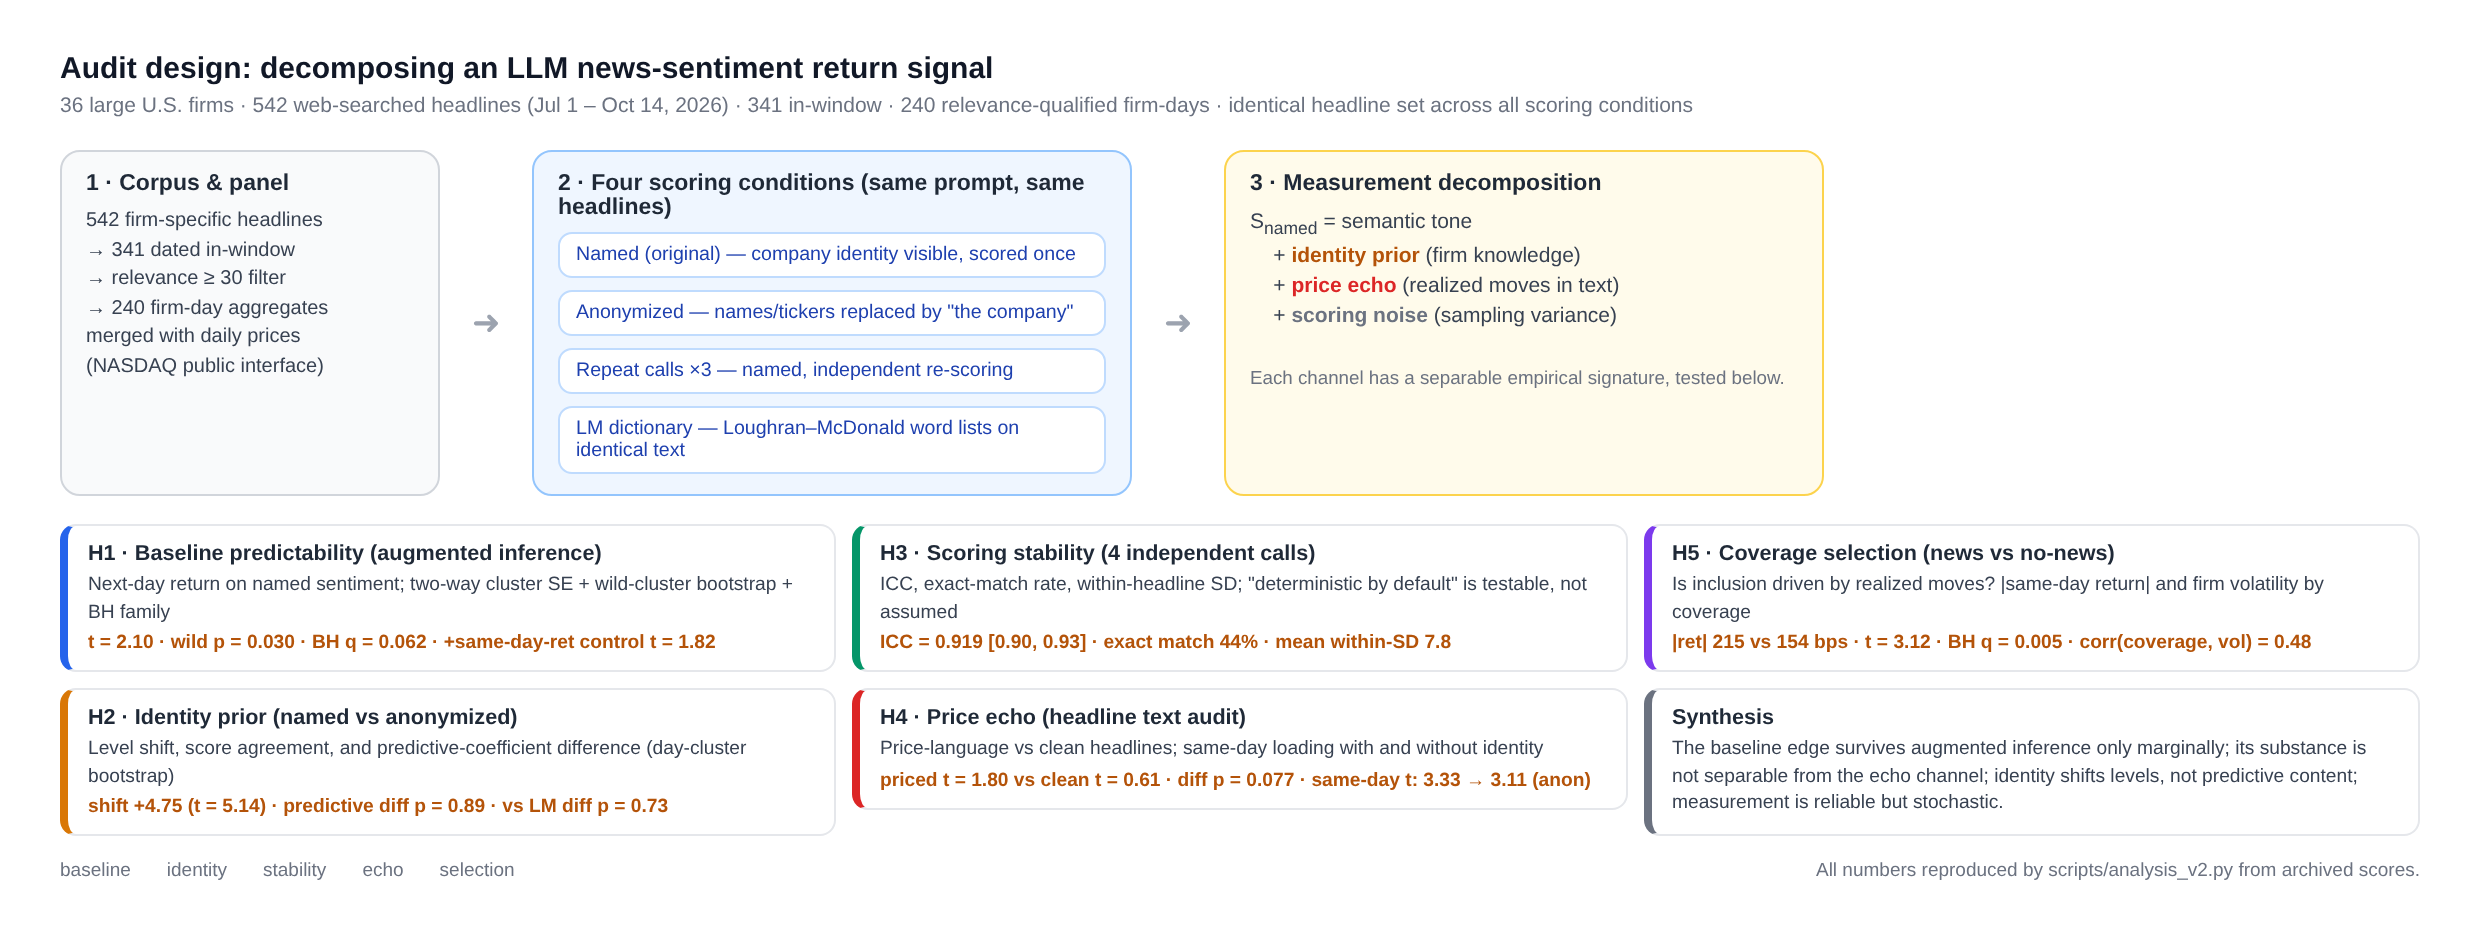
\includegraphics{../data/figures/fig_audit_design.png}
\end{adjustbox}
\caption{Audit design. One frozen corpus is scored under four conditions (named, anonymized, three repeat calls, dictionary), each isolating one term of the measurement decomposition $S=\kappa\theta+\iota G+\rho P+\varepsilon$; the five pre-specified hypotheses test the channels jointly under a common inference standard. All numbers are reproduced by \texttt{analysis\_v2.py} from archived scores.}
\label{fig:design}
\end{figure}
